\documentclass[12pt]{article}

\usepackage[utf8]{inputenc}
\usepackage{geometry}
\geometry{a4paper, margin=1in}
\usepackage{graphicx}
\usepackage{hyperref}
\usepackage{fancyhdr}

\setlength{\headheight}{15pt}
\pagestyle{fancy}
\fancyhf{}
\rhead{Computer Workshop Course}
\lhead{Final Assignment}
\rfoot{Page \thepage}

\title{
    \vspace{2in}
    \textbf{Final CW projrct :}\\
    \textbf{Integration of Tools and Practices}\\
    \large Iran University of Science and Technology\\
    \vspace{2in}
}

\author{
    \vspace{0.5in}
    Koosha Majlessi\\
    Computer Workshop\\
    \vspace{0.5in}
}

\begin{document}

\begin{titlepage}
    \maketitle
    \thispagestyle{empty}
\end{titlepage}

\newpage

\section{Git and GitHub}
\subsection{Repository Initialization and Commits}
First, we go to the GitHub website, click on the "New" option to create a new repository, and then use the terminal to clone it with the git clone command.

\subsection{GitHub Actions for LaTeX Compilation}
First, we create the main.yml file, commit it to GitHub and tag the commit.


\section{Exploration Tasks}
\subsection{Vim Advanced Features}
1. Jump Quickly Between Parentheses
If you're working with code that has lots of parentheses, brackets, or braces, you can jump between them using the precent sign.

2. Change Text Inside Parentheses or Quotes
With the ci command, you can quickly delete and replace text inside parentheses, quotes, or similar structures

3. Vim's Hidden Game!
Vim has a hidden game called Vim Adventure to help you practice commands. Type :help! to access it and explore while learning Vim.
\subsection{Memory profiling}
This semester, you got to know about dynamic memory allocation in C in your Programming Fundamentals class.

\subsubsection{Memory Leak}
A memory leak happens when a program allocates memory but doesn't free it, causing unused memory to remain reserved. It can occur if you forget to call free(), lose the reference to allocated memory, or don't handle errors properly. This leads to wasted memory and can slow down or crash the program.
\subsubsection{Memory profilers}
Valgrind is a tool used for detecting memory leaks, invalid memory accesses, and other memory-related issues in programs. It tracks memory allocations and deallocations, reporting any memory that was allocated but not freed. This helps developers identify and fix memory leaks, improving program reliability and performance.

\subsection{GNU/Linux Bash Scripting}
In this section, you will get to know some handy bash utilities.

\subsubsection{fzf}
Read about a handy CLI tool called \textit{fzf} and answer the following questions:

\begin{itemize}
    \item Fuzzy searching finds matches even with small differences or typos in the search term. It helps locate items by showing similar results, even if the search query is incomplete or misspelled.
    \item The command ls | fzf lists the files and directories in the current directory (ls), then passes that list through a pipe (|) to fzf, which performs fuzzy searching.
\end{itemize}

\subsubsection{Using fzf to find your favorite PDF}
1. Finding PDF Files
To list all files with the .pdf extension, you can use the following command:
fd -e pdf
Here, the fd command searches for all files with this extension in the current directory and its subdirectories.

2. Selecting a File Using fzf
To select a specific PDF file from the list of results, you can use the fzf tool. The following command accomplishes this:
fd -e pdf | fzf
At this point, the list of PDF files is passed to fzf, allowing you to navigate through the files using the arrow keys and select the desired file. This method is both efficient and user-friendly

\subsubsection{Opening the file using Zathura}
To open the selected PDF using Zathura, we can use the output of the commands mentioned earlier and pass it to Zathura. Here’s how to do it:
Command:
zathura dollar sign(fd -e pdf | fzf)
Explanation:
fd -e pdf: Lists all files with the .pdf extension.
| fzf: Passes the list of PDF files to fzf, allowing the user to select one file interactively.
dollar sign(command): Executes the command inside the parentheses and substitutes its output. Here, it takes the selected file path from fzf and passes it to zathura.
zathura dollar sign(...): Opens the selected PDF file in Zathura.
Usage:
When you run this command, a list of PDF files appears. Use the arrow keys to select the desired file and press Enter. The selected file will open in Zathura.

\section{Git and FOSS}
\subsection{README.md}
Make sure to include a basic README.md file in your GitHub repository that describes the aim of this repository and its purpose.

Make sure to use headings and lists in your README.md file.

\subsection{Issues}
Create sample issue. Screenshot in \ref{fig:issue}.
\begin{figure}[htbp]
    \centering
    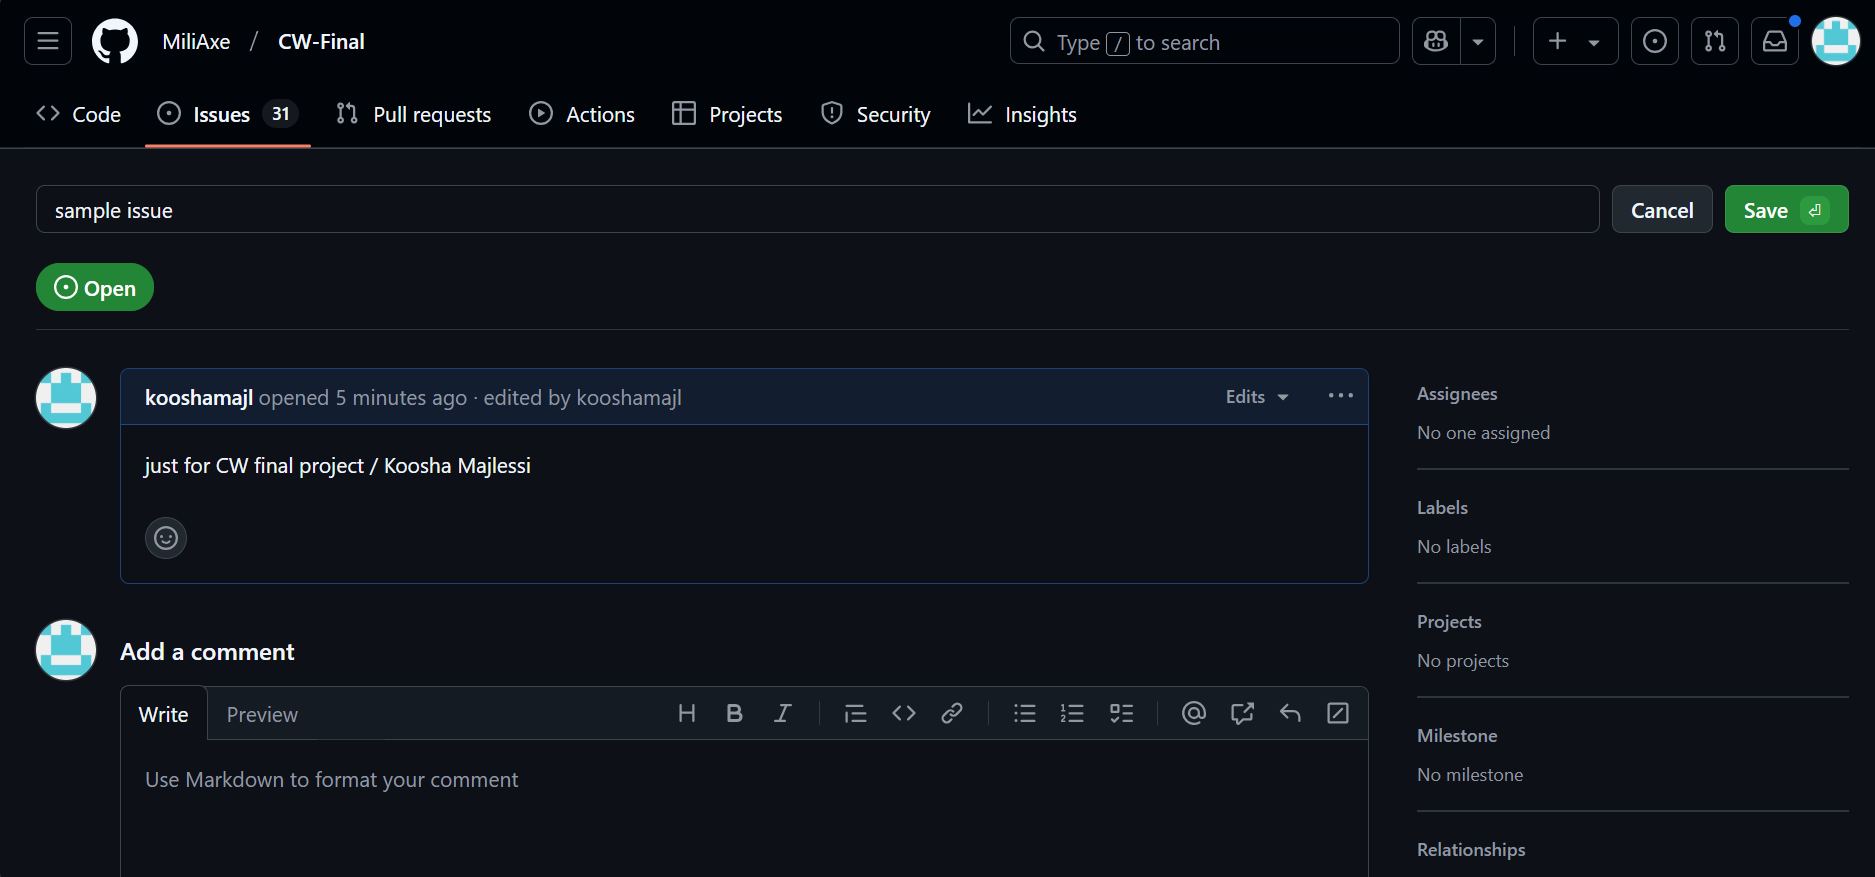
\includegraphics[width=0.5\textwidth]{pic/Screenshot 2025-01-19 235151.png}
    \caption{A screenshot of sample issue.}
    \label{fig:issue}
\end{figure}

\subsection{FOSS contribution}
I am passionate about developing FOSS because it allows me to improve my program with feedback from the community, bringing it to its best possible version.
\pagebreak

\end{document}